\documentclass[style=upen, size=14pt]{powerdot}
\definecolor{arany}{RGB}{255,242,0}
\hypersetup{backref=page}
\hypersetup{
    colorlinks=true,
    linkcolor=cyan,
    filecolor=magenta,      
    urlcolor=cyan}
\usepackage{graphicx}
\usepackage{amsmath}
\DeclareMathOperator*{\argmax}{argmax}
\DeclareMathOperator*{\argmin}{argmin}
\usepackage{amssymb}
\usepackage{stmaryrd}
\usepackage[latin2]{inputenc}
%\usepackage[magyar]{babel}
%\usepackage{euler}
\usepackage{tikz}
\usepackage{tikz-qtree}
\usepackage{tikz-dependency}
\usepackage{linguex}
\usepackage{amsthm}

\tikzset{every tree node/.style={align=center,anchor=north}}
%\usepackage{tabularx}
%\usepackage{threeparttable}
%\usepackage{color}
%\selectlanguage{english}
%\frenchspacing
\newcommand{\nd}{\noindent}
\newcommand{\Val}{\mathop{\mathit{Val}}}
\newcommand{\gold}{\color{arany}}
%\usepackage{tikz}
%\usepackage{tikz-qtree}
%\newcommand{\qed}{\hfill\mbox{\raggedright \rule{.1in}{.1in}}}
\def\es{\mathbin\land}
\theoremstyle{definition}
\newtheorem*{definition}{Definition}
\newtheorem{axioma}{Axiom}
\newtheorem{tetel}{Theorem}
\newtheorem{prop}{Proposition}
\newtheorem{lemma}{Lemma}
\begin{document}

\title{Natural Language Processing\\~~\\Lecture 4\\N-gram based language modeling}
% \author{}

\date{2021}
\maketitle

\begin{slide}[toc=What is an lm?]{What is a language model?}
  Recall that in formal language theory a language $\mathcal L$ is simply
  defined as a subset of $\Sigma^*$ for some alphabet $\Sigma$.\bigskip

  Statistical language models, in contrast, switch to a \emph{probabilistic
    view} of language production, and assign to any arbitrary
  $\langle w_1,\dots, w_n\rangle \in V^*$ sequence of tokens from the vocabulary
  $V$ a
  $$P(\langle w_1,\dots, w_n\rangle)$$ probability.
\end{slide}

\begin{slide}[toc=]{Vocabularies}
  Traditionally, the vocabulary of language models consisted of whole words,
  e.g.,
  \begin{center}
    $V$ = $\{$\emph{the}, \emph{be}, \emph{to}, \emph{of}, $\dots\}$
  \end{center}
  but more recently subword and character based language models have also been
  widely used, with vocabularies like $\{$ \emph{\_don'}, \emph{t}, \emph{\_un},
  \emph{related}, $\dots\}$ or $\{$\emph{a, b, c, d, e, f}, $\dots\}$.\bigskip

  This lecture discusses word based language modeling techniques -- techniques
  for character and subword level modeling are 
\end{slide}

\begin{slide}[toc=Why are LMs useful?]{Why are language models useful?}
  Probabilistic language models are important for a large number of NLP
  applications, in which the goal is to produce plausible word sequences as
  output, among them
  \begin{itemize}
  \item spell and grammar checking,
  \item predictive input,
  \item speech-to-text,
  \item chatbots,
  \item machine translation,
  \item summarisation.
  \end{itemize}
\end{slide}

\begin{slide}[toc=Continuations]{Modeling with continuation probabilities}
  Using the chain rule, the probability of a token sequence
  $\mathbf{w} = \langle w_1,\dots, w_n\rangle$ can be rewritten as
  $$P(\mathbf w)= P(w_1)\cdot P(w_2 \vert w_1 )\dots \cdot P(w_n\vert w_1,\dots, w_{n-1}),$$
  
  that is, for a full language model it is enough to specify
  \begin{itemize}
  \item[(i)] for any $w\in V$ word, the probability $P(w)$ that it will be the first
    word in a sequence, and
  \item[(ii)] for any $w\in V$
   and $\langle w_1,\dots,w_n\rangle$ partial sequence, the
  \emph{continuation probability} for $w$, that is,
  $$P(w ~\vert ~ w_1,\dots,w_n).$$
  \end{itemize}
\end{slide}


\begin{slide}[toc=Start and end symbols]{Start and end symbols}
  The chain rule based formulation of sequence probabilities
  \begin{itemize}
  \item requires a separate, unconditional clause for the starting probabilities, and 
  \item does not address the probability of \emph{ending} the sequence at a
    certain point.
  \end{itemize}
  Both issues can be solved by adding explicit $\langle$\textsc{start}$\rangle$
  and $\langle$\textsc{end}$\rangle$ symbols to the vocabulary, and assuming
  that all sequences of the language start/end with these. With this trick the
  starting/ending probabilities can be rewritten in conditional form as
  $P(w ~\vert~ \langle\textsc{start}\rangle)$ and
  $P(\langle\textsc{end}\rangle ~\vert~ \mathbf{w})$.
\end{slide}

\begin{slide}[toc=LM tree]{Language model tree structure}
  Using start/end symbols the word sequences with their continuation probabilities
  assigned by an LM can be arranged in a tree structure:
    \begin{center}
    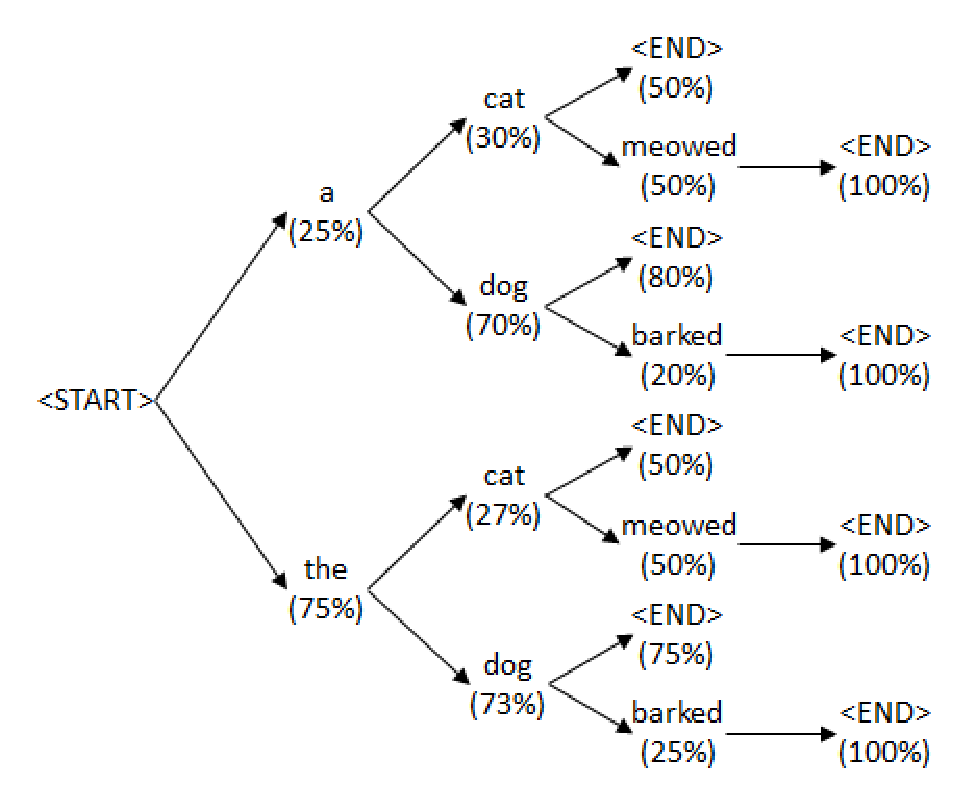
\includegraphics[width=0.6\textwidth]{figures/lm_tree.eps}
  \end{center}
\end{slide}

\begin{slide}[toc=Evaluation]{Evaluation}
  Language model evaluation can be
  \begin{itemize}
  \item \emph{\gold extrinsic}: how well does the model do as a component in a
    spell checker, speech-to-text system etc., or
  \item \emph{\gold intrinsic}: how well the assigned probabilities correspond
    to the texts in a test corpus?
  \end{itemize}
  The most widely used intrinsic evaluation metric is \emph{\gold perplexity} on
  a corpus. A language model $\mathcal M$'s perplexity over the sequence
  $\mathbf w = \langle w_1,\dots, w_n\rangle$ is
$$\mathbf{PP}_{\mathcal M}(\mathbf w) = \sqrt[n]{\frac{1}{P_{\mathcal M}(\mathbf w)}}.$$
\end{slide}

\begin{slide}[toc=]{Evaluation cont.}
  With the chain rule perplexity can be rewritten as

$${\sqrt[n]{\frac{1}{P_{\mathcal M}(w_1)}\cdot \frac{1}{P_{\mathcal M}(w_2 \vert w_1 )}\dots\cdot \frac{1}{P_{\mathcal M}(w_n\vert w_1,\dots, w_{n-1})}}}$$

which is exactly the \emph{geometric mean} of the reciprocals of the conditional
probabilities of all words in the corpus.\bigskip

In other, words, perplexity measures, ``how surprising'', on average, words are
(continuations) in the corpus for the language model.
\end{slide}

\begin{slide}[toc=]{Evaluation cont.}
  Taking the logarithm of perplexity, with a few simple steps of algebraic
  manipulations we can see that the result is

  $$
  - \frac{1}{n} \left(\log P_{\mathcal M}(w_1) + \sum_{i=2}^n\log P_{\mathcal M}(w_i ~\vert~ w_1,\dots, w_{i-1})\right),
$$

which is the average cross-entropy and negative log-likelihood per word. A
simple consequence: by minimizing average cross-entropy or maximizing average
log-likelihood one also minimizes the model's perplexitiy on the training data.
\end{slide}

\end{document}



%%% Local Variables:
%%% mode: latex
%%% TeX-master: t
%%% End:

% LocalWords:  Tokenization
